% =====================================================================
% FLAIR --- Seminar talk (~30-45 min, widescreen 16:9)
% Self-contained Beamer deck. Custom minimalist "FLAIR" theme so it needs
% only standard packages (beamer, xcolor, graphicx, booktabs).
% Figures embedded from figures/. Numbers match main_v3 (4 observed sites).
% Build: pdflatex clif_flair_talk.tex  (x2 for the frame counter)
% =====================================================================
\documentclass[aspectratio=169,11pt,xcolor={table}]{beamer}

\usepackage[T1]{fontenc}
\usepackage{lmodern}
\usepackage{graphicx}
\usepackage{booktabs}

\graphicspath{{figures/}}

% ---- FLAIR palette (RUSH ESM2 cohort scheme: charcoal / blue / red) --
\definecolor{flairink}{HTML}{1A1A1A}
\definecolor{flairmuted}{HTML}{6B6B6B}
\definecolor{flairpanel}{HTML}{F7F7F6}
\definecolor{flairgrid}{HTML}{E7E7E4}
\definecolor{flairblue}{HTML}{1A6FB2}      % clean blue  (48h series)
\definecolor{flairred}{HTML}{E0221C}       % strong red  (no-cap series)
\definecolor{flaircharcoal}{HTML}{3F3F3F}  % charcoal    (24h series)
\definecolor{nugreen}{HTML}{6F9E78}
\definecolor{ucmcviolet}{HTML}{8A6EA6}
\definecolor{flairband}{HTML}{F0E3DA}

% per-section accent cycles through the three cohort colors (blue / red / charcoal)
\newcommand{\secaccent}{\ifcase\value{section}flairblue\or flairblue\or flairred\or flaircharcoal\or flairblue\else flairblue\fi}

% ---- Minimalist theme ----------------------------------------------
\usetheme{default}
\usecolortheme{default}
\setbeamertemplate{navigation symbols}{}
\setbeamercolor{normal text}{fg=flairink}
\setbeamercolor{structure}{fg=flairblue}
\setbeamercolor{frametitle}{fg=flairink}
\setbeamercolor{title}{fg=flairink}
\setbeamercolor{itemize item}{fg=flairblue}
\setbeamercolor{itemize subitem}{fg=flairmuted}
\setbeamercolor{block title}{fg=white,bg=flairblue}
\setbeamercolor{block body}{bg=flairpanel}
\setbeamerfont{frametitle}{series=\bfseries,size=\Large}
\setbeamerfont{title}{series=\bfseries}
\setbeamertemplate{itemize item}{\small\raisebox{0.15ex}{\textbullet}}
\setbeamertemplate{itemize subitem}{\scriptsize\raisebox{0.15ex}{--}}
\setbeamertemplate{blocks}[rounded][shadow=false]

% frame title rule
\setbeamertemplate{frametitle}{%
  \vskip0.6em%
  \begin{beamercolorbox}[wd=\paperwidth,leftskip=0.9em,rightskip=0.9em]{frametitle}%
  \usebeamerfont{frametitle}\insertframetitle%
  \ifx\insertframesubtitle\empty\else{\\[0.1em]\small\color{flairmuted}\insertframesubtitle}\fi%
  \vskip0.25em{\expandafter\color\expandafter{\secaccent}\rule{0.10\paperwidth}{2.2pt}}%
  \end{beamercolorbox}%
}

% footline: short title | frame number
\setbeamertemplate{footline}{%
  \hbox{\begin{beamercolorbox}[wd=\paperwidth,ht=2.2ex,dp=1.0ex,leftskip=0.9em,rightskip=0.9em]{}%
  \color{flairmuted}\scriptsize FLAIR: Federated ICU Benchmark on CLIF \hfill \insertframenumber%
  \end{beamercolorbox}}%
}

\newcommand{\emphc}[1]{{\color{flairblue}\textbf{#1}}}
\newcommand{\rushc}[1]{{\color{flairred}\textbf{#1}}}
\newcommand{\source}[1]{{\par\vskip0.3em\scriptsize\color{flairmuted}#1}}

% section divider frames
\AtBeginSection[]{%
  \begin{frame}[plain]
  \vfill
  \centering
  {\expandafter\color\expandafter{\secaccent}\rule{0.14\paperwidth}{3pt}}\\[0.8em]
  {\usebeamerfont{title}\Large\color{flairink}\insertsectionhead}\\[0.4em]
  \vfill
  \end{frame}%
}

% ---- Title metadata -------------------------------------------------
\title{\textbf{FLAIR}}
\subtitle{A Federated ICU Benchmark for External Validation\\ on the Common Longitudinal ICU Format}
\author{CLIF Consortium \textperiodcentered\ FLAIR Working Group}
\date{\today}

\begin{document}

% ===================== TITLE =========================================
\begin{frame}[plain]
  \vfill
  {\color{flairblue}\rule{0.16\paperwidth}{4pt}}\\[1.1em]
  {\usebeamerfont{title}\Huge\color{flairink} FLAIR}\\[0.35em]
  {\large\color{flairblue}\textbf{F}ederated \textbf{L}earning \textbf{A}ssessment for \textbf{I}CU \textbf{R}esearch}\\[0.8em]
  {\Large\color{flairink} A Federated ICU Benchmark for External Validation}\\[0.2em]
  {\Large\color{flairmuted} on the Common Longitudinal ICU Format (CLIF)}\\[1.4em]
  {\color{flairmuted} CLIF Consortium \textperiodcentered\ FLAIR Working Group}\\[0.3em]
  {\small\color{flairmuted} \today}
  \vfill
  \begin{flushright}\scriptsize\color{flairmuted}
    MIMIC-CLIF \textperiodcentered\ Rush \textperiodcentered\ Northwestern \textperiodcentered\ UChicago Medicine
    \quad\textbullet\quad 278{,}065 ICU stays
  \end{flushright}
\end{frame}

% ===================== ONE-LINE FRAMING ==============================
\begin{frame}{The question in one line}
  \vfill
  \begin{center}
  {\Large A model that looks strong on public ICU data ---}\\[0.5em]
  {\Large does it still work at a hospital that \emphc{did not build it}?}
  \end{center}
  \vfill
  \begin{center}\color{flairmuted}
  FLAIR is the federated infrastructure that answers this, reproducibly,\\
  without moving a single patient record.
  \end{center}
  \vfill
\end{frame}

\section{The gap}

% ===================== HOOK ==========================================
\begin{frame}{Evidence for ICU AI does not keep pace with models}
  \begin{columns}[T]
  \begin{column}{0.54\textwidth}
    \begin{itemize}
      \item Models for sepsis, extubation, mortality appear \emphc{continually}
      \item Whether one works \emph{outside} its development hospital is often \emphc{unknown}
      \item The evidence gap is an \emphc{access gap}: representative multi-site ICU data rarely reach the team that must test the model
    \end{itemize}
  \end{column}
  \begin{column}{0.44\textwidth}
    \begin{block}{A cautionary anchor}
      The Epic Sepsis Model --- deployed across many US hospitals --- fell to \rushc{AUC 0.63} on independent external evaluation, against vendor-claimed 0.76--0.83.
    \end{block}
    \source{Wong et al., JAMA Intern Med 2021; Habib et al. 2021}
  \end{column}
  \end{columns}
  \vfill
  {\color{flairmuted}\small Sepsis Watch and TREWS each took \emph{years} to reach a handful of sites --- serious validation does not scale.}
\end{frame}

% ===================== BENCHMARKS SATURATE ===========================
\begin{frame}{Public benchmarks help --- but cannot close the gap alone}
  \begin{itemize}
    \item MIMIC, eICU, HiRID, YAIB, EHRSHOT are essential for \emphc{reproducible development}
    \item But they \emphc{centralize their test data} --- and so:
    \begin{itemize}
      \item inherit one source's selection biases
      \item can \emph{saturate}: tuning against the same public set makes transport look easier than it is
    \end{itemize}
    \item None offers a standing, ICU-scoped, \emphc{federated validation} layer over data that never leaves the hospital
  \end{itemize}
  \vfill
  \begin{center}\color{flairblue}\textbf{Develop on public MIMIC-CLIF \quad$\rightarrow$\quad validate federated.}\end{center}
  \source{van de Water et al. 2023 (YAIB); Wornow et al. 2023 (EHRSHOT); Arnrich et al. 2025 (MEDS)}
\end{frame}

% ===================== BENCHMARKS: WHAT THEY MISS =====================
\begin{frame}{What current ICU benchmarks measure --- and miss}
  \begin{itemize}
    \item Tasks cluster on \emphc{mortality, length-of-stay, and physiologic deterioration} (AKI, sepsis) --- even multi-center YAIB stays within mortality / AKI / sepsis / kidney / LOS
    \item Sparse on \emphc{deployment decisions}: disposition (LTACH), extubation failure, readmission, and \emphc{leak-safe before-treatment} sepsis (CDC ASE)
    \item \emphc{Global / random splits, not temporal} --- no pseudo-prospective, deployment-time estimate
    \item Centralized (or single-site, e.g.\ EHRSHOT $=$ one Stanford site) test data --- external multi-site validation is not built in, and benchmarks saturate
    \item Row-level metrics, not \emph{operational} (one alarm per stay)
  \end{itemize}
  \vfill
  \begin{center}\color{flairblue}\textbf{They measure discrimination on public data --- not whether a model \emph{survives deployment} at a new hospital.}\end{center}
  \source{van de Water et al.\ 2023; Wornow et al.\ 2023; Harutyunyan et al.\ 2019}
\end{frame}

% ===================== RELATED MODEL-TO-DATA EFFORTS ==================
\begin{frame}{Related model-to-data efforts --- pieces of the answer}
  \begin{itemize}
    \item \emphc{OHDSI / LEGEND} --- federated network studies over OMOP (share SQL / coefficients)
    \item \emphc{OpenSAFELY} --- analytic code to national primary-care data; no patient rows move
    \item \emphc{MedPerf} --- model-to-data benchmarking, largely imaging
    \item \emphc{FeTS} --- federated \emph{training} for imaging
    \item \emphc{DREAM / EHR DREAM} --- model-to-data evaluation as a \emph{challenge}
  \end{itemize}
  \vfill
  \begin{center}\color{flairmuted}
  Missing for ICU EHR: a \emphc{standing, ICU-scoped federated benchmark} on a critical-care standard.
  \end{center}
  \begin{center}\color{flairblue}\textbf{FLAIR combines a critical-care standard (CLIF) $+$ a reusable task catalog $+$ a standing federated protocol.}\end{center}
  \source{Guinney et al. 2018 (DREAM); Bergquist et al. 2024 (EHR DREAM); OpenSAFELY 2021; Karargyris et al. 2023 (MedPerf); Pati et al. 2022 (FeTS); Reps et al. 2020 (OHDSI/LEGEND)}
\end{frame}

% ===================== FLAIR = 3 ARTIFACTS ===========================
\begin{frame}{FLAIR = three coupled artifacts}
  \begin{columns}[T]
  \begin{column}{0.33\textwidth}
    \begin{block}{Data layer}
      CLIF critical-care standard; public \emphc{MIMIC-CLIF} entry point ($\sim$72{,}800 stays)
    \end{block}
  \end{column}
  \begin{column}{0.33\textwidth}
    \begin{block}{Task layer}
      Five inspectable Python tasks; \emphc{open, PR-extensible} catalog
    \end{block}
  \end{column}
  \begin{column}{0.33\textwidth}
    \begin{block}{Protocol layer}
      Committee-reviewed, \emphc{aggregate-only} model-to-data execution
    \end{block}
  \end{column}
  \end{columns}
  \vfill
  \begin{center}
  {\large The model goes to the data. \quad Only aggregate, cell-suppressed reports come back.}
  \end{center}
  \vfill
  {\color{flairmuted}\small Not a clinical-utility claim --- an \emph{evidence layer} between local development and any clinician-facing decision.}
\end{frame}

% ===================== PUBLIC BENCHMARKS vs FLAIR =====================
\begin{frame}{Public benchmarks vs FLAIR}
  \begin{center}
  \scriptsize
  \setlength{\tabcolsep}{5pt}
  \rowcolors{2}{flairpanel}{white}
  \begin{tabular}{>{\raggedright\arraybackslash}p{2.5cm}>{\raggedright\arraybackslash}p{4.3cm}>{\raggedright\arraybackslash}p{4.3cm}}
  \toprule
  \textbf{Dimension} & \textbf{Public ICU benchmarks} & \textbf{FLAIR} \\
  \midrule
  Test data & centralized / single-site & \emphc{federated}, stays at each hospital \\
  Tasks & mortality, LOS, AKI, sepsis (generic) & 5 \emphc{deployment} tasks: LTACH disposition, extubation failure, before-treatment CDC-ASE sepsis, readmission, mortality \\
  Train/test split & global / random & \emphc{temporal} (pseudo-prospective) at external sites \\
  External validation & same repository / pooled & \emphc{independently governed} hospitals \\
  Scoring & row-level & episodic / landmark / peak (\emphc{operational}) \\
  Task catalog & fixed & \emphc{PR-extensible} \\
  \bottomrule
  \end{tabular}
  \end{center}
  \vfill
  {\color{flairmuted}\small Complementary, not competing: \emphc{develop} on public benchmarks, \emphc{validate} federated on FLAIR.}
  \source{van de Water et al. 2023 (YAIB); Wornow et al. 2023 (EHRSHOT); Pollard et al. 2018 (eICU); Harutyunyan et al. 2019}
\end{frame}

\section{Methods}

% ===================== DATA LAYER ====================================
\begin{frame}{Data layer: CLIF and MIMIC-CLIF}
  \begin{itemize}
    \item \emphc{CLIF} harmonizes ICU EHR content into shared relational tables with mCIDE category definitions (vitals, labs, meds, respiratory support, microbiology, ADT, \dots)
    \item Task code refers to \emphc{shared table names and category values} --- portable across sites, minimal per-site feature engineering
    \item \emphc{MIMIC-CLIF} expresses MIMIC-IV in CLIF v2.1 ($\sim$72{,}800 ICU stays) --- the public development set
  \end{itemize}
  \vfill
  \begin{center}\color{flairblue}\textbf{Develop on public MIMIC-CLIF \quad$\rightarrow$\quad validate on private CLIF data.}\end{center}
  \source{Rojas et al. 2025 (CLIF); Johnson et al. 2023 (MIMIC-IV)}
\end{frame}

% ===================== DATA ACCESS: 3 WAYS ===========================
\begin{frame}{Three ways to get data out of CLIF}
  \begin{columns}[T]
  \begin{column}{0.33\textwidth}
    \begin{block}{1. Direct feature extraction}
      Compute features straight from the CLIF tables --- the reference baseline's path (count features over an ELF vocabulary).
    \end{block}
  \end{column}
  \begin{column}{0.33\textwidth}
    \begin{block}{2. MEDS format \emph{(optional)}}
      Export as a standardized Medical Event Data Standard event stream for MEDS-native pipelines.
    \end{block}
  \end{column}
  \begin{column}{0.33\textwidth}
    \begin{block}{3. Wide dataset}
      A YAIB-style wide tabular matrix for models that expect one row of features per prediction.
    \end{block}
  \end{column}
  \end{columns}
  \vfill
  \begin{center}\color{flairmuted}
  MEDS is \emphc{one option}, not a required step --- a model developer picks whichever representation fits.
  \end{center}
  \source{Arnrich et al. 2025 (MEDS); van de Water et al. 2023 (YAIB); Wornow et al. 2023 (EHRSHOT/FEMR)}
\end{frame}

% ===================== FIVE TASKS ====================================
\begin{frame}{Task layer: five ICU prediction tasks}
  \begin{center}
  \footnotesize
  \setlength{\arrayrulewidth}{0.4pt}
  \rowcolors{2}{flairpanel}{white}
  \begin{tabular}{llllc}
  \toprule
  \textbf{Task} & \textbf{Outcome} & \textbf{Grid} & \textbf{Mode} & \textbf{Prev.} \\
  \midrule
  T1 & ICU daily mortality        & daily 07:00      & landmark & 0.125 \\
  T2 & LTACH discharge            & daily 07:00      & landmark & 0.062 \\
  T3 & Extubation failure 24\,h   & at extubation    & episodic & 0.054 \\
  T4 & Sepsis (CDC ASE) 6\,h      & hourly           & peak     & 0.061 \\
  T5 & Unplanned ICU readmission  & at ICU discharge & episodic & 0.093 \\
  \bottomrule
  \end{tabular}
  \end{center}
  \vfill
  \begin{itemize}\small
    \item One Python module per task: \texttt{META} + \texttt{build()} $\rightarrow$ one row per prediction opportunity
    \item Spans outcome, disposition, respiratory, infectious-deterioration, utilization
    \item Catalog \emphc{grows by contribution}: acceptance needs MIMIC reproducibility, clinician face validity, $\geq$2-site sign-off
  \end{itemize}
\end{frame}

% ===================== T4 SEPSIS =====================================
\begin{frame}{Task 4 is sepsis by the \emph{surveillance} definition}
  \begin{columns}[T]
  \begin{column}{0.58\textwidth}
    \begin{itemize}
      \item \emphc{CDC Adult Sepsis Event (ASE)} within 6\,h, hourly, hospital-wide
      \item $t_0$ = earliest ASE criterion (blood culture, qualifying antibiotics, vasopressor, organ dysfunction) via \texttt{clifpy.utils.ase}
      \item Prediction window ends \emphc{strictly before} $t_0$ --- no label leakage from treatment
      \item Follows the \emph{before-treatment} formulation; contrasts with antibiotic-anchored Sepsis-3
    \end{itemize}
  \end{column}
  \begin{column}{0.40\textwidth}
    \begin{block}{Why it matters}
      A rare, hospital-wide, hourly screen --- the most clinically consequential task, and the most fragile under distribution shift.
    \end{block}
  \end{column}
  \end{columns}
  \source{Kamran et al., NEJM AI 2024; Rhee et al. 2019 (CDC ASE)}
\end{frame}

% ===================== SAFEGUARDS ====================================
\begin{frame}{Three safeguards make cohorts comparable across sites}
  \begin{enumerate}
    \item \emphc{Stitched hospitalizations.} Fragmented episodes (ED$\to$inpatient, discharge$\to$rapid readmit) joined into one \texttt{hospitalization\_join\_id} (6\,h gap) --- one episode is the unit, never split across train/test
    \item \emphc{Strict point-in-time.} Features use only data at or before \texttt{prediction\_dttm} --- the no-future-data boundary
    \item \emphc{Audit hash.} A SHA-256 over task source + policy metadata is stamped into every report
  \end{enumerate}
  \vfill
  \begin{center}\color{flairblue}\textbf{Sites can prove they ran byte-identical task code.}\end{center}
\end{frame}

% ===================== DATA SPLITS ===================================
\begin{frame}{Data splits: pseudo-prospective by design}
  \begin{columns}[T]
  \begin{column}{0.56\textwidth}
    \begin{itemize}
      \item \emphc{75/25} split at the \emphc{stitched-hospitalization} grain --- one hospitalization never straddles the boundary
      \item \emphc{Default = temporal split}: oldest 75\% train, newest 25\% test
      \item Estimates \emphc{pseudo-prospective performance} --- how the frozen model behaves \emph{going forward in time}, without a prospective trial
      \item \emphc{MIMIC-CLIF is the exception}: de-identified admission dates carry no usable time order $\rightarrow$ deterministic hash split
    \end{itemize}
  \end{column}
  \begin{column}{0.42\textwidth}
    \begin{block}{Consequence}
      At external sites, degradation blends \emph{temporal} shift (train-past $\to$ test-future) with \emph{cross-site} shift --- both are what a new hospital actually faces.
    \end{block}
  \end{column}
  \end{columns}
\end{frame}

% ===================== BASELINE ======================================
\begin{frame}{Reference baseline: one frozen, shippable model}
  \begin{itemize}
    \item \emphc{XGBoost} over point-in-time \emphc{count features} (EHRSHOT/FEMR tradition)
    \item CLIF events $\rightarrow$ fixed \emphc{211-code} ELF vocabulary; counts of codes strictly before prediction time
    \item Units never features; discharge diagnoses excluded (no leakage)
    \item HPO once on MIMIC-CLIF (\emphc{Optuna}, 30 trials, 5-fold CV AUROC)
    \item Model + dictionary \emphc{shipped unchanged} to sites for \emph{inference only} --- no per-site training
  \end{itemize}
  \vfill
  {\color{flairmuted}\small A benchmark check, not a claim that the baseline is clinically adequate. It exists to expose transport behavior.}
  \source{Wornow et al. 2023; Steinberg et al. 2021 (FEMR)}
\end{frame}

% ===================== EVAL MODES + REPORT ===========================
\begin{frame}{Three evaluation modes --- and what each report contains}
  \begin{center}
  \scriptsize
  \setlength{\tabcolsep}{5pt}
  \rowcolors{2}{flairpanel}{white}
  \begin{tabular}{>{\raggedright\arraybackslash}p{1.5cm}>{\raggedright\arraybackslash}p{2.9cm}>{\raggedright\arraybackslash}p{6.6cm}}
  \toprule
  \textbf{Mode} & \textbf{Prediction unit} & \textbf{Report bundle} \\
  \midrule
  \emphc{Episodic}\newline (T3, T5) & one prediction per stay & AUROC, AUPRC, ROC \& PR curves, \emphc{calibration} (slope / intercept / Brier + reliability), \emphc{decision-curve analysis}, subgroup AUROC \\
  \emphc{Landmark}\newline (T1, T2) & one per daily landmark & per-landmark $\widehat{\mathrm{AUC}}(t)$ \emph{curve} \emphc{plus} a single \emphc{pooled dynamic AUC}; lead-time / skill plots \\
  \emphc{Peak}\newline (T4) & stay collapsed to max risk & discrimination + subgroup only; \emphc{calibration \& DCA omitted} (the ``peak-calibration trap'') \\
  \bottomrule
  \end{tabular}
  \end{center}
  \vfill
  {\color{flairmuted}\small Every bundle also carries a cohort summary, a suppressed-code registry, and audit metadata. All metrics on the held-out test split; percentile-bootstrap 95\% CIs at the \emph{stay} level.}
\end{frame}

% ===================== POOLED DYNAMIC AUC FORMULA ====================
\begin{frame}{The landmark metric: pooled dynamic AUC}
  \small
  For a stitched hospitalization $h$ with event onset $T_h$, discharge $D_h$, horizon $\tau$, at landmark time $t$:
  \vskip0.3em
  \begin{columns}[T]
  \begin{column}{0.5\textwidth}
    \setlength{\abovedisplayskip}{2pt}\setlength{\belowdisplayskip}{4pt}
    Risk set (still admitted, event-free):
    \[ R(t)=\{\,h : T_h>t,\ D_h>t\,\} \]
    Dynamic label (event within $\tau$):
    \[ Y_h(t)=\mathbf 1\{\,t<T_h\le t+\tau\,\} \]
    Predicted risk from history $\mathcal H_h(t)$:
    \[ p_h(t)=\hat P\!\left(t<T_h\le t+\tau \mid \mathcal H_h(t)\right) \]
    Tie kernel: $\ \psi(a,b)=\mathbf 1\{a>b\}+\tfrac12\mathbf 1\{a=b\}$
  \end{column}
  \begin{column}{0.5\textwidth}
    \setlength{\abovedisplayskip}{2pt}\setlength{\belowdisplayskip}{4pt}
    Time-specific AUC:
    \[ \resizebox{\linewidth}{!}{$\displaystyle \widehat{\mathrm{AUC}}(t)=\frac{\sum_{i,j\in R(t)}Y_i(t)\,[1-Y_j(t)]\,\psi\big(p_i(t),p_j(t)\big)}{\big(\sum_i Y_i(t)\big)\big(\sum_j [1-Y_j(t)]\big)}$} \]
    Pooled across landmarks (\emphc{reported}):
    \[ \resizebox{\linewidth}{!}{$\displaystyle \mathrm{AUC}_{\text{pooled}}=\frac{\sum_t \widehat{\mathrm{AUC}}(t)\,w_t}{\sum_t w_t},\ \ w_t=\text{cases}_t\!\cdot\!\text{controls}_t$} \]
  \end{column}
  \end{columns}
  \vskip0.2em
  \begin{center}
  {\scriptsize\color{flairmuted}$h$ hospitalization \textbullet\ $t$ landmark \textbullet\ $\tau$ horizon \textbullet\ $T_h$ onset \textbullet\ $D_h$ discharge\\
  $R(t)$ risk set \textbullet\ $Y_h(t)$ label \textbullet\ $p_h(t)$ risk \textbullet\ $\psi$ tie kernel \textbullet\ $w_t$ case--control pairs at $t$}
  \end{center}
  \source{Heagerty \& Zheng 2005; van Houwelingen 2007; Blanche et al.\ 2013}
\end{frame}

% ===================== PROTOCOL / WORKFLOW ===========================
\begin{frame}{Protocol layer: the model-to-data loop}
  \begin{center}
    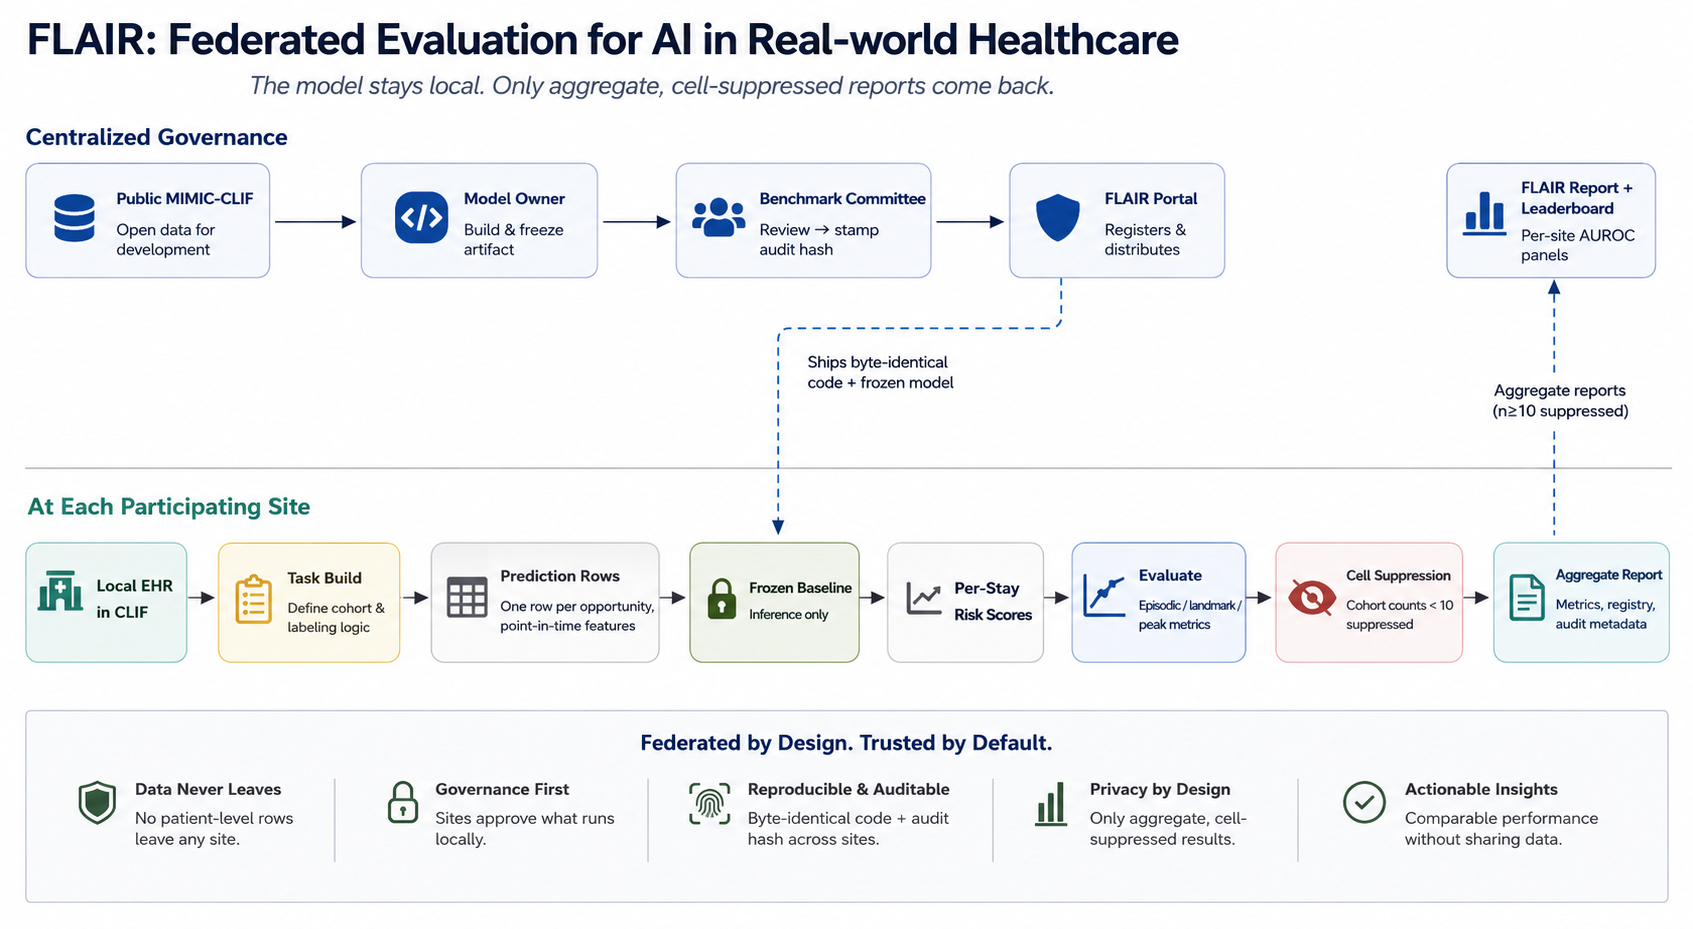
\includegraphics[width=\linewidth]{figure1_flair_overview.png}
  \end{center}
  {\centering\scriptsize\color{flairmuted} Centralized governance (top): MIMIC-CLIF $\rightarrow$ Model Owner $\rightarrow$ Committee (audit hash) $\rightarrow$ Portal. At each site (bottom): frozen baseline runs locally; only aggregate, cell-suppressed reports return.\par}
\end{frame}

% ===================== GOVERNANCE ====================================
\begin{frame}{Privacy and governance are operational, not aspirational}
  \begin{itemize}
    \item \emphc{No patient-level data leave any site}
    \item \emphc{Cell suppression} enforced by the library: cohort counts $<10$ suppressed; subgroups $<10$ omitted; sparse calibration bins withheld
    \item \emphc{Governance precedes execution} --- committee review; sites keep final approval over what runs locally
    \item Every report carries: discrimination, calibration/DCA (where applicable), subgroup + lead-time summaries, suppressed code registry, and \emphc{audit metadata}
  \end{itemize}
  \vfill
  {\color{flairmuted}\small Model-to-data lineage of DREAM / EHR DREAM --- FLAIR makes it a \emph{standing ICU benchmark}.}
\end{frame}

\section{Results}

% ===================== COHORT ========================================
\begin{frame}{Four sites reporting; four onboarding}
  \begin{center}
  \footnotesize
  \rowcolors{2}{flairpanel}{white}
  \begin{tabular}{lrrrr}
  \toprule
  \textbf{Site} & \textbf{ICU stays} & \textbf{F\%} & \textbf{Age} & \textbf{SOFA} \\
  \midrule
  MIMIC-CLIF & 72{,}778 & 43.2 & 67 & 5 \\
  Rush & 53{,}356 & 47.8 & 63 & 4 \\
  Northwestern Medicine & 114{,}335 & 44.0 & 66 & 5 \\
  UChicago Medicine & 37{,}596 & 43.5 & 61 & 6 \\
  \rowcolor{white} Consortium sites 5--8 & --- & --- & --- & --- \\
  \bottomrule
  \end{tabular}
  \end{center}
  \vfill
  \begin{center}\large\color{flairblue}\textbf{278{,}065 ICU stays across four independent health systems.}\end{center}
  {\color{flairmuted}\small Placeholder rows leave space for the full eight-site consortium --- no fabricated numbers.}
\end{frame}

% ===================== HEADLINE FOREST ===============================
\begin{frame}{The headline: per-site discrimination, one panel per task}
  \begin{center}
    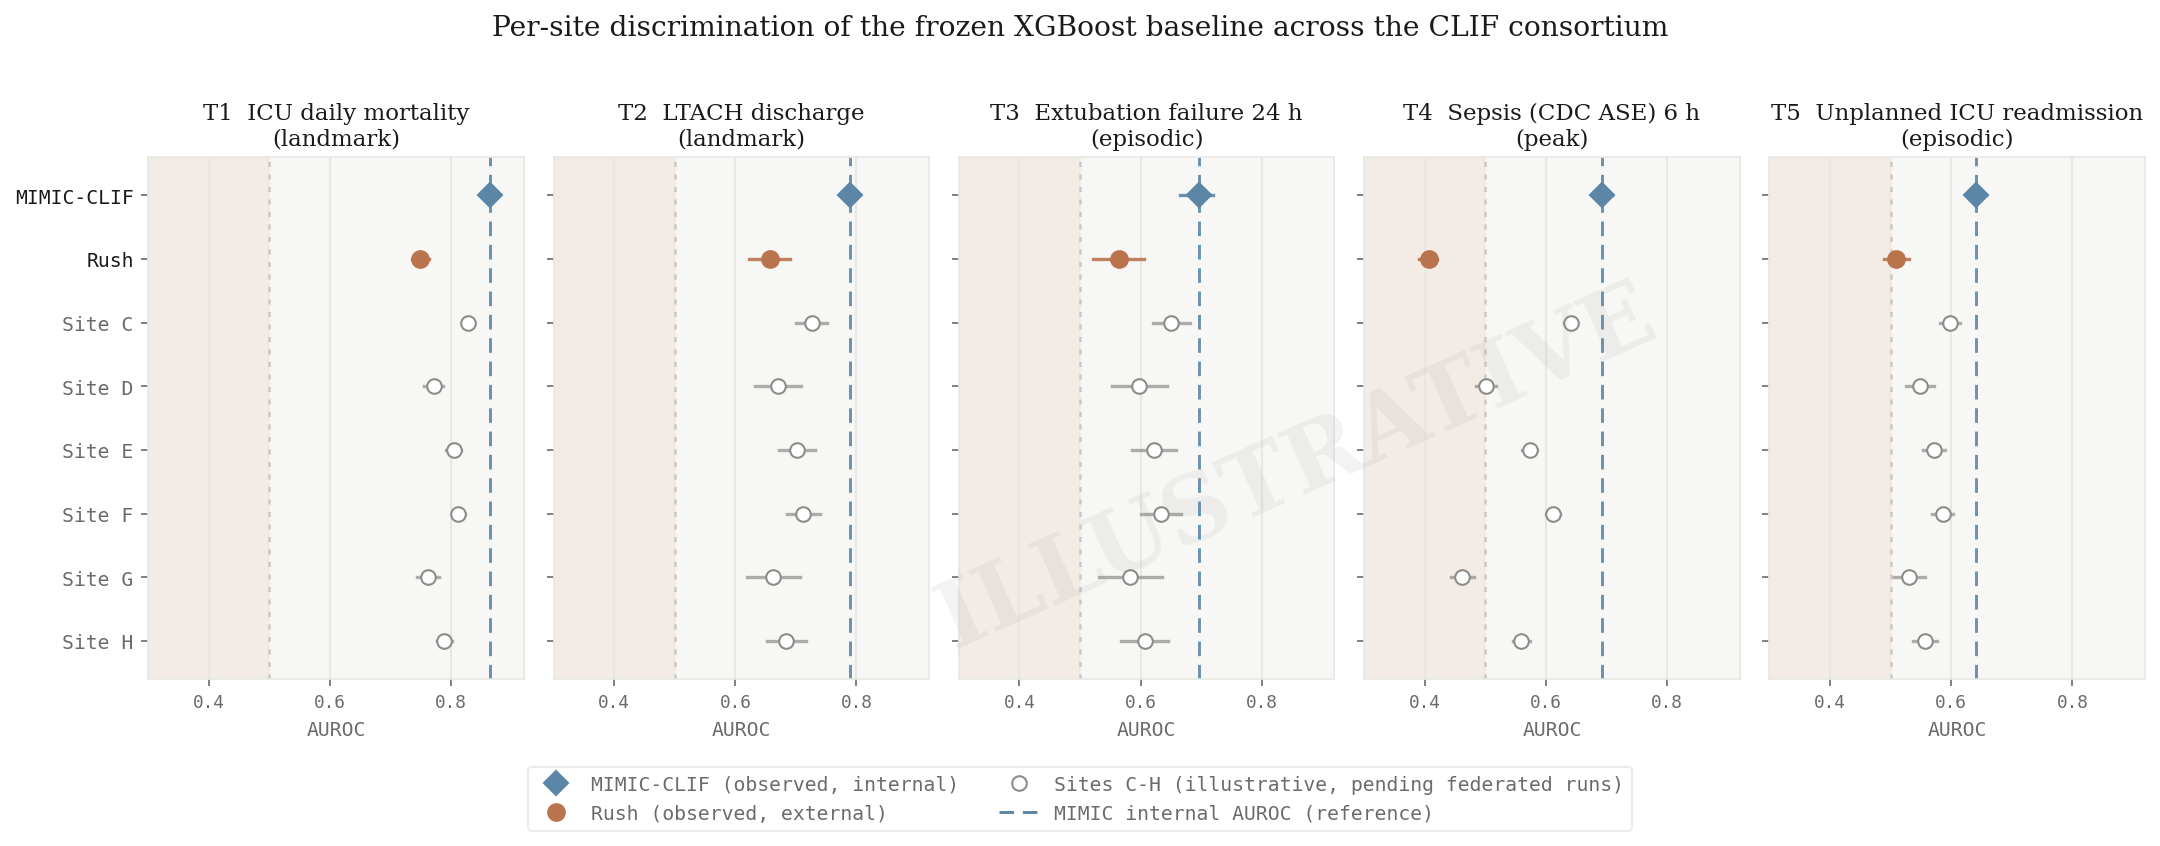
\includegraphics[width=0.98\linewidth]{figure2_forest_auroc.png}
  \end{center}
  \vskip-0.3em
  {\color{flairmuted}\small A single pooled AUROC would hide this. The per-site \emph{spread} is the point.}
\end{frame}

% ===================== DEGRADATION ===================================
\begin{frame}{Strong internal discrimination does not survive transport}
  \begin{columns}[c]
  \begin{column}{0.62\textwidth}
    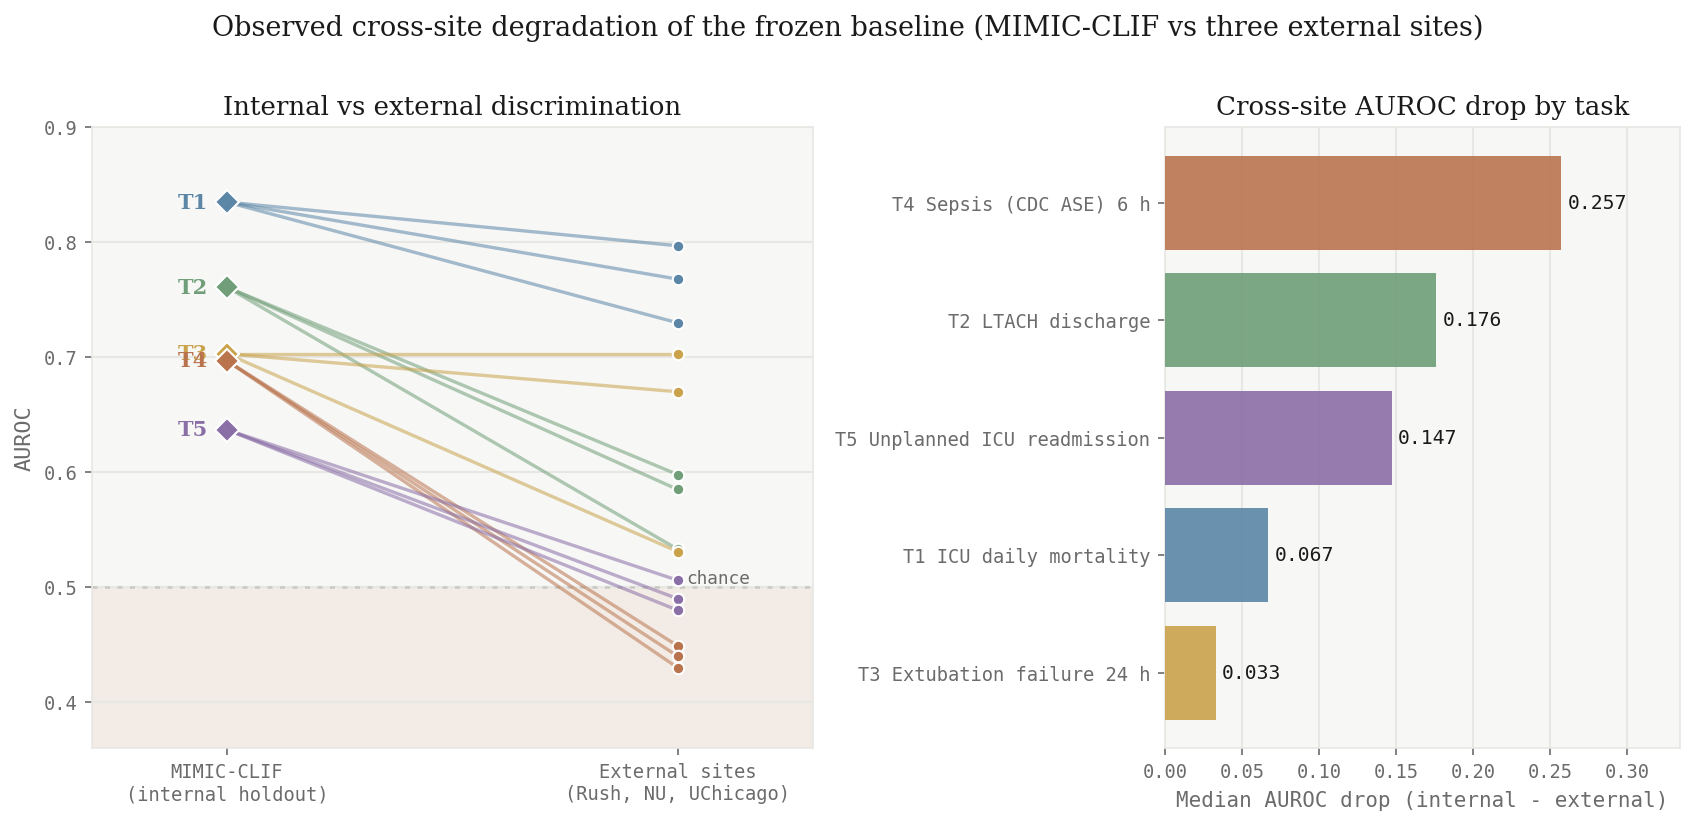
\includegraphics[width=\linewidth]{figure3_degradation.png}
  \end{column}
  \begin{column}{0.36\textwidth}
    \small Median internal$\to$external AUROC drop:
    \begin{itemize}\small
      \item Sepsis \rushc{0.257}
      \item LTACH \phantom{0}0.176
      \item Readmission 0.147
      \item Mortality 0.067
      \item Extubation 0.033
    \end{itemize}
    \emphc{Task-dependent}, not uniform.
  \end{column}
  \end{columns}
\end{frame}

% ===================== SEPSIS BELOW CHANCE ===========================
\begin{frame}{Sepsis falls \emph{below chance} at every external site}
  \vfill
  \begin{center}
  \large
  \begin{tabular}{lc}
    MIMIC-CLIF (internal) & \emphc{0.697} \\[0.3em]
    Rush & \rushc{0.430} \\
    Northwestern Medicine & \rushc{0.449} \\
    University of Chicago Medicine & \rushc{0.440} \\
  \end{tabular}
  \end{center}
  \vfill
  \begin{center}
  {\large The reproducible external result on the highest-stakes task is a model}\\
  {\large that is \rushc{worse than a coin flip}.}
  \end{center}
  \vfill
  {\color{flairmuted}\small Not a one-hospital artifact --- three independent health systems, same failure.}
\end{frame}

% ===================== TASK-DEPENDENT NARRATIVE ======================
\begin{frame}{Transportability is task-dependent --- and heterogeneous}
  \begin{columns}[T]
  \begin{column}{0.33\textwidth}
    \begin{block}{Transports}
      \textbf{Mortality (T1)}\\ external 0.73--0.80\\ vs 0.835 internal
    \end{block}
  \end{column}
  \begin{column}{0.33\textwidth}
    \begin{block}{Collapses}
      \textbf{Sepsis (T4)}\\ below chance everywhere\\ \textbf{Readmission (T5)}\\ $\approx$ chance
    \end{block}
  \end{column}
  \begin{column}{0.33\textwidth}
    \begin{block}{Splits}
      \textbf{Extubation (T3)}\\ Northwestern \emphc{0.703}\\ (ties MIMIC)\\ UChicago \rushc{0.531}
    \end{block}
  \end{column}
  \end{columns}
  \vfill
  \begin{center}
  {\large The within-task, across-site spread is exactly what federated external validation exists to surface.}
  \end{center}
\end{frame}

\section{Discussion}

% ===================== SATURATION / EVIDENCE LAYER ===================
\begin{frame}{Why federate evaluation --- and why now}
  \begin{itemize}
    \item \emphc{Saturation resistance.} Test data stay siloed --- the leaderboard's data never enter public hands, limiting pretraining-on-the-test-set and tune-to-test incentives
    \item \emphc{Evaluation, not training.} Aggregate cell-suppressed metrics leak less than the model updates exchanged in federated \emph{learning}; no per-site model object to share
    \item \emphc{Re-inspectable.} Byte-identical code + audit hashes make cohort definitions, exclusions, and labels auditable across sites
  \end{itemize}
  \vfill
  \begin{center}\color{flairblue}\textbf{An evidence layer between local development and any clinician-facing claim.}\end{center}
\end{frame}

% ===================== LIMITATIONS ===================================
\begin{frame}{Limitations}
  \begin{itemize}\small
    \item Depends on \emphc{CLIF adoption} --- unmapped sites need an ETL step first
    \item Structured EHR + binary classification only --- no notes, waveforms, images, or treatment effects
    \item \emphc{Aggregate-only} reporting limits fine-grained error analysis; suppressed small subgroups invisible centrally
    \item Evaluates \emphc{frozen} models --- no federated training
    \item Four sites today (four onboarding); each external site uses a \emph{temporal} split, so some degradation may reflect temporal as well as cross-site shift
  \end{itemize}
\end{frame}

% ===================== CONCLUSION ====================================
\begin{frame}{Takeaways}
  \begin{enumerate}
    \item FLAIR federates ICU \emphc{evaluation} on a shared critical-care standard (CLIF) --- model-to-data, aggregate-only, auditable
    \item A frozen public-data baseline already exposes \emphc{large, task-dependent} cross-site degradation across \emphc{four} real health systems
    \item \emphc{Sepsis} discrimination falls \emph{below chance} at every external site; \emphc{mortality} transports; \emphc{extubation} splits by site
    \item The contribution is not a model --- it is a \emphc{reproducible way to ask} whether ICU models behave alike across institutions
  \end{enumerate}
  \vfill
  \begin{center}\Large\color{flairblue}\textbf{Develop on public MIMIC-CLIF. Validate federated.}\end{center}
\end{frame}

% ===================== THANK YOU =====================================
\begin{frame}[plain]
  \vfill
  \centering
  {\color{flairblue}\rule{0.14\paperwidth}{3pt}}\\[0.9em]
  {\Huge\color{flairink}\textbf{Thank you}}\\[0.8em]
  {\large\color{flairmuted} FLAIR --- Federated Learning Assessment for ICU Research}\\[0.4em]
  {\small\color{flairmuted} github.com/clif-consortium/FLAIR}\\[1.2em]
  {\footnotesize\color{flairmuted} MIMIC-CLIF \textperiodcentered\ Rush \textperiodcentered\ Northwestern \textperiodcentered\ UChicago Medicine \quad\textbullet\quad 278{,}065 ICU stays}
  \vfill
\end{frame}

\end{document}
